\documentclass[a4paper]{article}

\usepackage[francais]{babel}
\usepackage[utf8]{inputenc}
\usepackage[T1]{fontenc}
\usepackage{listings}
\usepackage{xcolor}
\usepackage{fullpage}
\usepackage{graphicx}


\definecolor{mygreen}{rgb}{0,0.6,0}
\definecolor{mygray}{rgb}{0.5,0.5,0.5}
\definecolor{mymauve}{rgb}{0.58,0,0.82}

\lstset{
  backgroundcolor=\color{white},   % choose the background color; you must add
                                   % \usepackage{color} or \usepackage{xcolor}
  basicstyle=\ttfamily,              % the size of the fonts that are used for
                                   % the code
  breakatwhitespace=false,         % sets if automatic breaks should only happen
                                   % at whitespace
  breaklines=true,                 % sets automatic line breaking
  captionpos=b,                    % sets the caption-position to bottom
  commentstyle=\itshape\color{purple!40!black},    % comment style
  deletekeywords={...},            % if you want to delete keywords from the
                                   % given language
  escapeinside={\%*}{*)},          % if you want to add LaTeX within your code
  extendedchars=true,              % lets you use non-ASCII characters; for
                                   % 8-bits encodings only, does not work with
                                   % UTF-8
  frame=single,                       % adds a frame around the code
  identifierstyle=\color{blue},
  keepspaces=true,                 % keeps spaces in text, useful for keeping
                                   % indentation of code (possibly needs
                                   % columns=flexible)
  keywordstyle=\bfseries\color{green!40!black},       % keyword style
  language=C,                      % the language of the code
  otherkeywords={*,...},           % if you want to add more keywords to the set
  numbers=left,                    % where to put the line-numbers; possible
                                   % values are (none, left, right)
  numbersep=5pt,                   % how far the line-numbers are from the code
  numberstyle=\tiny\color{mygray}, % the style that is used for the line-numbers
  rulecolor=\color{black},         % if not set, the frame-color may be changed
                                   % on line-breaks within not-black text
                                   % (e.g. comments (green here))
  showspaces=false,                % show spaces everywhere adding particular
                                   % underscores; it overrides
                                   % 'showstringspaces'
  showstringspaces=false,          % underline spaces within strings only
  showtabs=false,                  % show tabs within strings adding particular
                                   % underscores
  stepnumber=2,                    % the step between two line-numbers. If it's
                                   % 1, each line will be numbered
  stringstyle=\color{orange},     % string literal style
  tabsize=2,                       % sets default tabsize to 2 spaces
  title=\lstname                   % show the filename of files included with
                                   % \lstinputlisting; also try caption instead
                                   % of title
}

\newcommand{\boardsize}{\ensuremath{\mathtt{BOARD\_SIZE}}}

\title{ARCSYS2 TP noté : 7 colors}
\author{Simon Bihel, Corentin Ferry}
\date{Mars 2016}

\begin{document}
    \maketitle

    \section{Introduction}
    Dans ce rapport nous présentons notre travail pour le TP noté d'ARCSYS sur 
    le jeu \emph{7 colors}. 
    
    Il s'agissait de réaliser un jeu des 7 couleurs, où le but de chaque joueur 
est d'obtenir plus de cases que son adversaire sur un plateau à cases colorées.
Chaque joueur choisit, lorsque vient son tour, une couleur et absorbe les cases 
adjacentes à sa zone qui sont de cette couleur. Il répète cette opération 
jusqu'à ce qu'il ne puisse plus obtenir de nouvelles cases, et c'est alors à 
l'adversaire de jouer.
    
    En plus des questions obligatoires, nous avons réalisé une IA hégémonique, 
une IA AlphaBeta et aussi un meilleur affichage pour le terminal.

    L'ensemble des fonctions que nous avons écrites sont documentées au-dessus 
de leur implémentation, dans le fichier .c qui les contient. Les fonctions 
relatives aux règles du jeu sont dans \texttt{7colors.c}, les fonctions 
relatives à l'entrée/sortie et au déroulement du jeu sont dans \texttt{game.c}, 
les fonctions relatives à l'intelligence articifielle sont dans \texttt{ai.c}.
Le format de la documentation est \emph{Javadoc}.

    \section{Partie 2 : Voir le monde en 7 couleurs}
    \paragraph{Question 2.1}
    Nous avons implémenté une fonction permettant de remplir le monde avec
des couleurs aléatoires, représentées par un \texttt{char} dont la valeur est
comprise entre \texttt{65} (\texttt{A}) et \texttt{72} (\texttt{G}).
Le prototype de cette fonction est le suivant :
\begin{lstlisting}
void fill_board(char* board)
\end{lstlisting}
On utilise dans cette fonction le générateur de nombres aléatoires de la
\texttt{libc}, que l'on suppose préalablement initialisé à l'aide de la
fonction \texttt{srand()}.

    \paragraph{Question 2.2}

    Nous avons implémenté la fonction \texttt{update\_board} sous le prototype 
qui suit :
\begin{lstlisting}
int update_board(char* board, char player, char color)
\end{lstlisting}
Elle procède à la mise à jour du plateau par double boucle, en attribuant au 
joueur \texttt{player} les cases voisines des siennes, qui sont de la couleur 
\texttt{color}.
Cette opération est répétée jusqu'à ce que plus aucune case du plateau ne soit 
changée.

Compte tenu de la structure de cette fonction, on peut s'assurer qu'elle fait 
bien ce que l'on cherche (autrement dit, que la coloration de proche en proche 
est bien effectuée) en remplissant le plateau d'une seule couleur. Le premier 
joueur à choisir cette couleur devrait alors s'attribuer l'ensemble des cases 
du plateau, sauf celle de départ de son adversaire. 

C'est d'ailleurs ce cas-là qui est le pire relativement à la complexité 
temporelle : c'est celui qui comporte le plus de cases à colorier en un seul 
tour, et surtout, c'est un cas tel qu'il existe une suite de cases adjacentes 
de même couleur entre la case de départ d'un joueur et celle de l'autre, qui 
sont les cases les plus éloignées du plateau.

Dans ce cas, le monde va être mis à jour par lignes ou colonnes successives 
(selon le point 
de départ) en partant du joueur qui a choisi la bonne couleur, comme sur la 
figure \ref{update_board}.
\begin{figure}
	\centering
	
	\includegraphics[width=.45\columnwidth]{update_board_arcsys_1} \\
	\vspace{1cm}
	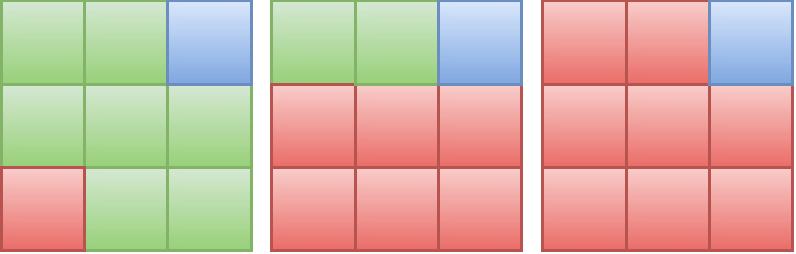
\includegraphics[width=.45\columnwidth]{update_board_arcsys_2}
	
	\caption{\label{update_board} Deux cas d'actualisation du plateau dans 
le pire cas. En haut, le joueur bleu absorbe les cases vertes, colonne par 
colonne. En bas, le joueur rouge absorbe les cases vertes, ligne par ligne.}
\end{figure}

Alors, il y aura $\boardsize-1$ passes à effectuer, où \boardsize{} est la 
taille du plateau. 

    \paragraph{Question 2.3}
    Nous n'avons pas réécrit la fonction précédente. Néanmoins, on peut 
proposer une implémentation de type \emph{flood-fill}~: il s'agirait de 
procéder récursivement au remplissage des cases, en partant de la case de 
départ du joueur courant.

Pour chaque case parcourue, on regarde si celle-ci appartient au joueur ou est 
de la couleur cible. Si c'est le cas, on parcourt les cases adjacentes, dans 
deux directions, en s'éloignant de la case de départ (pour éviter de passer 
plusieurs fois sur des cases déjà visitées). Il serait nécessaire d'implémenter 
un système de marquage; nous avons utilisé cette technique à la question 6.1.

    \section{Partie 3 : À la conquête du monde}
    \paragraph{Question 3.1} Compte tenu du fait que nous allions devoir 
écrire des stratégies de jeu automatiques, nous avons écrit la fonction 
\texttt{game()} dont la structure permet de choisir la méthode de jeu de chaque 
joueur. Les fonctions de stratégies auxquelles \texttt{game()} fait appel 
renvoient toutes un \texttt{char} qui est la couleur choisie par le joueur. La 
bonne fonction à appeler est déterminée par une structure de contrôle de type 
\texttt{switch/case}.

Nous avons donc écrit une fonction \texttt{ask()}, dont le rôle est de demander 
à l'utilisateur la couleur qu'il a choisi de jouer. 

Notre implémentation évite les dépassements de buffer en récupérant un seul 
caractère via la fonction \texttt{getchar()}; tant que celui-ci n'est pas dans 
l'intervalle des 7 couleurs permises, on demande à nouveau à l'utilisateur de 
choisir une couleur.

Compte tenu de la simplicité de la fonction \texttt{ask()}, nous n'avons pas 
relevé de limite particulière qui lui serait imputable; elle remplit simplement 
son rôle.
    \paragraph{Question 3.2}
    Nous avons choisi la condition suffisante d'arrêt suivante : \textbf{le jeu 
peut s'arrêter lorsque l'un des deux joueurs a obtenu strictement plus de 50\% 
des cases.}

Cette condition d'arrêt a été implémentée à l'aide de compteurs de cases. La 
fonction de mise à jour du plateau, \texttt{update\_board()}, renvoie le nombre 
de case gagnées par le joueur en cours : la valeur de son compteur est alors 
incrémentée. Lorsque l'un des deux joueurs a plus de la moitié des cases du 
plateau, le jeu s'arrête.

L'affichage du pourcentage de cases occupées par chaque joueur est effectué 
après chaque tour à l'aide de la fonction \texttt{printf()}.
    \section{Partie 4 : La stratégie de l'aléa}
    % Simon
    \paragraph{Question 4.1} 
Il s'agit de la première stratégie automatisée que nous avons créée. La 
fonction \texttt{game()} y fait appel.

Nous avons implémenté une fonction de choix aléatoire de couleur. Elle se 
base sur la fonction \texttt{rand()} de la \texttt{libc}. On choisit un nombre 
aléatoire avec \texttt{rand()} entre 0 et 7 inclus, en utilisant un modulo, et 
on ajoute 65 pour arriver sur des caractères entre `A' et `G' inclus. 

Le résultat, de type \texttt{int}, est soumis à un \emph{cast} vers le type 
\texttt{char} avant d'être renvoyé.

    \paragraph{Question 4.2} 
    Pour jouer un coup aléatoirement en étant sûr d'ajouter des cases à la 
zone du joueur, on parcourt le plateau pour savoir de quelles couleurs sont les 
cases adjacentes à cette zone. 

Ensuite, on choisit aléatoirement une couleur à l'aide de \texttt{rand() \% 
7} et on la renvoie si un coup ajoutant des cases à la zone du joueur est 
possible avec; sinon, on choisit à nouveau une couleur aléatoirement.

    \section{Partie 5 : La loi du plus fort}
    \paragraph{Question 5.1}
    
    Nous avons implémenté une stratégie de jeu dans laquelle le joueur cherche 
à obtenir le plus de cases permises à chaque tour de jeu. Pour ce faire, on 
travaille sur une copie du plateau générée à l'aide de \texttt{memcpy()}, sur 
laquelle on simule le jeu d'une couleur à l'aide de la fonction 
\texttt{update\_board()}. On choisit alors une des couleurs pour laquelle le 
résultat renvoyé par \texttt{update\_board()} est maximal, autrement dit une de 
celles qui a permis d'obtenir le plus de cases.

Le plateau de jeu est rétabli entre chaque couleur essayée, en ré-effectuant 
une copie du plateau original avec \texttt{memcpy()}.

Le prototype de cette stratégie est : 
\begin{lstlisting}
char biggest_move(char* board, char player)
\end{lstlisting}

    \paragraph{Question 5.2}
    Nous avons fait s'affronter le joueur articifiel aléatoire et le joueur 
glouton. Il est apparu que le joueur glouton a gagné avec 52.11\% des cases 
contre 25.78\% pour le joueur aléatoire. Le joueur glouton augmente strictement 
son aire à chaque tour, ce qui n'est pas le cas du joueur aléatoire. 
Ceci constitue une première explication au score obtenu.

Nous avons choisi de réaliser un plateau équitable en le rendant symétrique. 
Ainsi, tant que la stratégie d'un joueur ne dépend pas des cases de l'autre, 
deux stratégies équivalentes choisies progressent exactement de la même 
manière. Dans cette situation, le joueur jouant en premier a toutefois un 
avantage : à stratégie équivalente, celui-ci aura un tour d'avance sur son 
adversaire et emportera la partie.
    \paragraph{Question 5.3}
    Nous avons effectué un championnat de 100 parties, entre le joueur 
artificiel glouton et le joueur aléatoire. L'intégralité des parties a été 
remportée par le joueur glouton. En effectuant 15 championnats successifs, le 
joueur aléatoire n'a pas remporté une seule partie. Il n'a pas dépassé les 30\% 
de terrain acquis par partie, ce qui le laisse loin de l'obtention d'une 
victoire.

Cela confirme l'observation que nous avions eue précédemment : la stratégie 
aléatoire n'est décrite par aucune rège, lorsque la stratégie gloutonne va 
maximiser son aire à chaque tour. Vu la règle du jeu, il est normal que la 
deuxième l'emporte su la première.

    \section{Partie 6 : Les nombreuses huitièmes merveilles du monde}
    % Corentin pour 6.1
    \paragraph{Question 6.1}
    Nous avons implémenté un joueur artificiel hégémonique. Il joue selon la 
stratégie de jeu suivante : il calcule l'aire atteignable par l'adversaire avec
un algorithme de propagation de type \emph{flood-fill}.

Cet algorithme de propagation est récursif : si une case est atteignable par un 
joueur, c'est-à-dire occupée par lui ou non occupée, alors on regarde ce qu'il 
en est de ses cases voisines (pour autant que celles-ci n'aient pas été 
visitées). Les cases visitées sont mises à une valeur qui n'est pas une 
couleur, ainsi l'algorithme travaille sur une copie du plateau de jeu.

Il n'y a alors qu'à compter le nombre de cases atteignables par l'autre joueur 
lors de l'exécution de l'algorithme de \emph{flood-fill}.

Nous avons effectué un championnat de 100 parties entre le joueur hégémonique 
et le joueur glouton. Les statistiques sur 15 parties sont situées figure 
\ref{hegemon_greedy}.


\begin{figure}
\centering

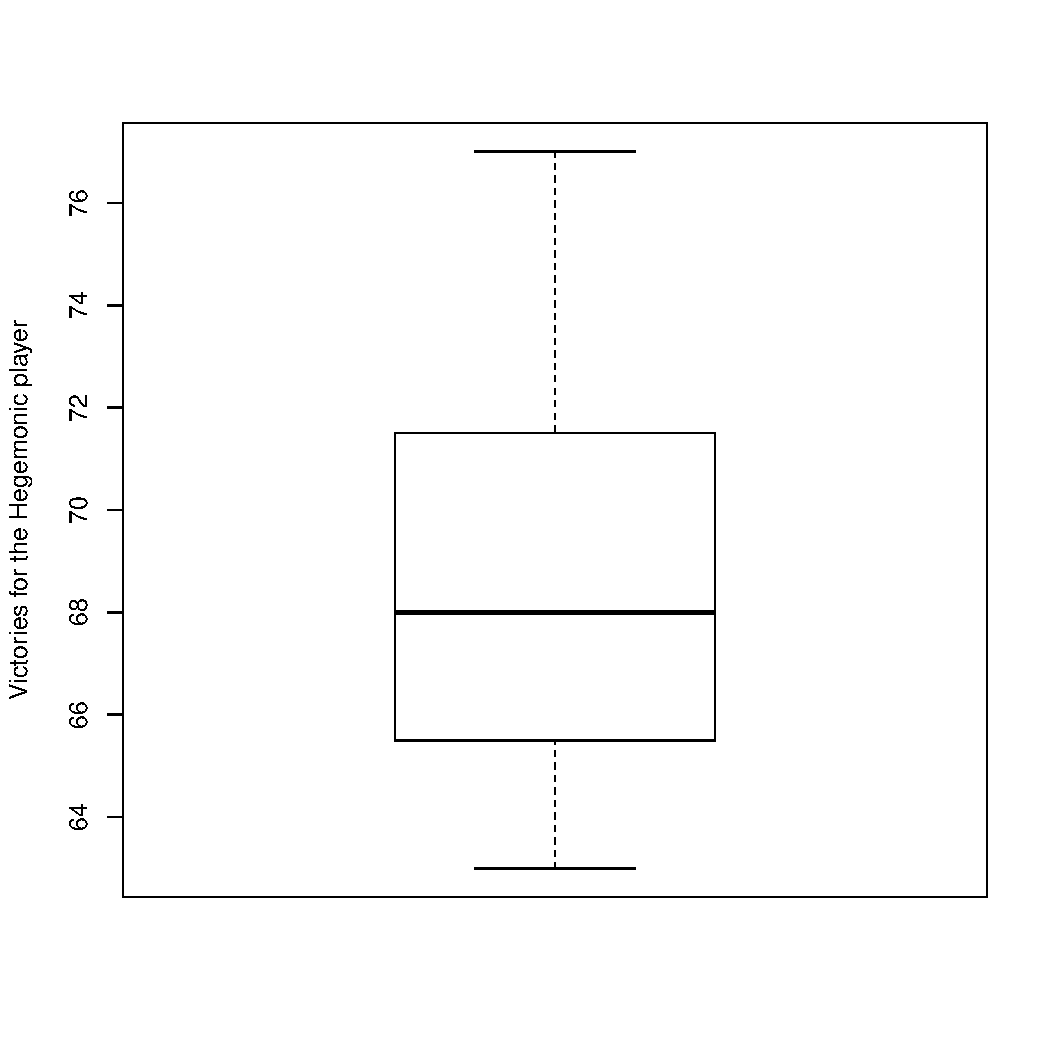
\includegraphics[width=.45\columnwidth]{hegemon_vs_greedy}
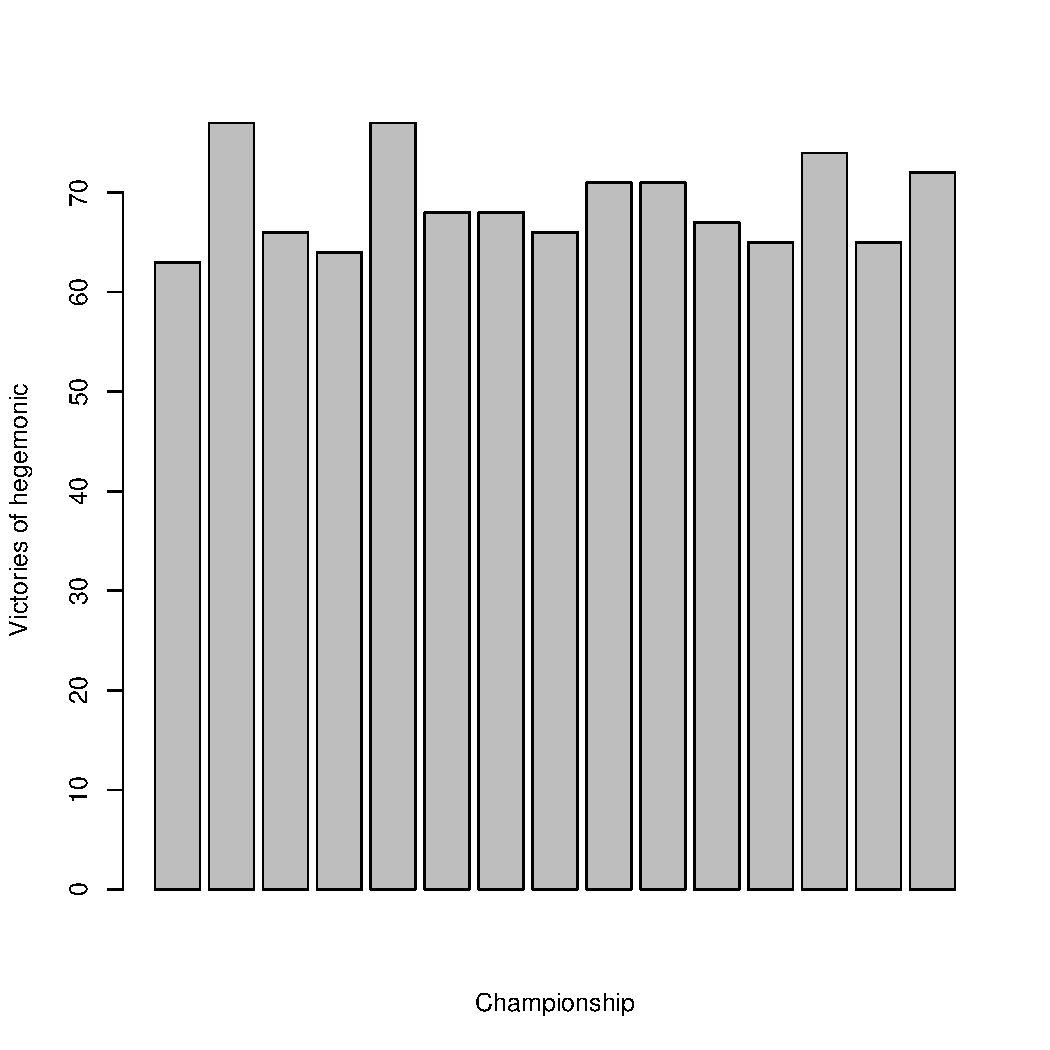
\includegraphics[width=.45\columnwidth]{hegemon_vs_greedy_bar}

\caption{\label{hegemon_greedy} À droite, le nombre de victoires remportées par 
l'algorithme glouton et par championnat. À gauche, les minima, maxima, moyenne 
et écart-type.}
\end{figure}

    \paragraph{Question 6.2} Nous sommes directement partis sur un algorithme 
MinMax, cet algorithme étant classique. Nous avons choisi le score comme
    heuristique. Comme on teste chaque couleur pour chaque joueur, la complexité
    est dans le pire cas en $O(7^n)$ où $n$ est le nombre de coups prévus. En 
pratique, la complexité est moindre, car si un coup ne change pas le score du 
joueur courant, alors on n'explore pas les coups qui le suivent. 
Aussi, pour chaque coup, on simule l'avancement de la partie~: on travaille 
donc sur une copie du plateau. 

Nous avons ensuite mis en place un algorithme AlphaBeta qui rajoute quelques 
conditions pour éviter de parcourir des coups qui conduisent à coup sûr à la 
défaite : on choisira d'arrêter l'exploration de l'arbre dès lors que le score 
maximal que le joueur en cours peut atteindre, est inférieur au score minimal 
que le joueur adverse peut atteindre. Une telle situation est en effet synonyme 
de défaite.


    \section{Partie 7 : Le pire du monde merveilleux des 7 couleurs}
    % Simon
    \paragraph{Question 7.2} Nous avons utilisé AlphaBeta en utilisant comme
    heuristique la fonction qui calcule l'aire disponible pour le joueur
    adverse. Nous l'avons nommé AlphaBeta hégémonique.
    
    Sur 100 parties contre l'ancien AlphaBeta et avec pour les
    deux joueurs un nombre des coups prévus\footnote{profondeur d'exploration} 
de 6, AlphaBeta hégémonique en gagna 71. 

Notons que AlphaBeta hégémonique était le joueur qui commençait. En 
inversant les rôles, AlphaBeta hégémonique gagna 56 parties. En mettant l'IA 
hégémonique simple à la place d'AlphaBeta normal, AlphaBeta hégémonique gagna 93 
parties.

Ces résultats s'expliquent par le fait que la stratégie hégémonique est 
meilleure que la stratégie gloutonne, et, pour AlphaBeta hégémonique contre 
l'hégémonique simple, le fait que AlphaBeta a une vision à plus long terme 
qu'une stratégie comme l'hégémonique.

    \section{Partie 8 : Pour procrastiner}
    % Simon
    \paragraph{Meilleur affichage} Nous avons amélioré l'affichage dans le
    terminal en utilisant des couleurs, et en affichant le plateau au-dessus du
    précédent (en l'écrasant) pour éviter le défilement. 
    
    Cela a été fait avec des codes d'échappement ANSI.

    \section{Conclusion}
    Nous avons programmé un jeu de 7 couleurs ainsi que de multiples stratégies 
de jeu automatisées. 
    
    S'agissant des résultats obtenus, IA hégémoniques et AlphaBeta 
se sont montrées meilleures que de simples IA gloutonnes. De plus, l'alliance 
des deux s'est aussi montrée supérieure.

Les résultats obtenus ne sont pas surprenants : lorsque la stratégie gloutonne 
ne voit que le gain immédiat, MinMax et AlphaBeta ont une vision à plus long 
terme : ils peuvent anticiper le score sur plusieurs étapes. La stratégie 
hégémonique est meilleure que la gloutonne au sens où elle ne va pas essayer de 
combler d'éventuels trous dans la zone du joueur, lorsque la stratégie 
gloutonne va maximiser l'aire du joueur, en comblant éventuellement ces trous.

La combinaison des deux stratégies gagnantes, à savoir la méthode hégémonique 
utilisée en tant qu'heuristique de AlphaBeta, donne une meilleure stratégie.

Un point qui mérite d'être soulevé indépendamment du jeu est 
le fait que '\texttt{valgrind} affiche une fuite de mémoire, constante, de 900 
octets, soit la taille d'un plateau. Cela signifie qu'un des plateaux créés n'a 
pas été libéré; une exploration profonde du code permettrait de trouver où la 
libération n'a pas été effectuée.

Nous n'avons pas implémenté d'interface graphique fenêtrée, qui utilise X11. 
Ceci constitue une évolution possible du jeu, pour permettre une interaction 
avec la souris, et une familiarisation avec l'usage de librairies externes, 
comme \texttt{libsdl}, \texttt{libsfml}.

    
\end{document}
